\section{Clases e Interfaces de package Retrofit}

En esta sección, se presenta una visualización de las clases e interfaces que componen el paquete `RetroFit`, el cual es esencial para la comunicación de la aplicación móvil con los servidores backend. Tal como se muestra en la Figura \ref{fig:Diagrama_app_movil_detallado} (en la sección de Estructura Interna Detallada de la Aplicación Móvil), este paquete encapsula toda la lógica de interacción con las APIs remotas.

El enfoque principal de esta sección es mostrar las clases e interfaces que definen cómo la aplicación se comunica con el Servidor Java Spring-Boot y el Servidor Red Neuronal. Estas imágenes proporcionan una representación visual directa del código, facilitando la comprensión de la estructura y las relaciones entre los diferentes componentes del paquete `RetroFit`.

A continuación, se mostrarán las imágenes de las clases e interfaces que conforman el paquete `RetroFit`. Cada imagen representa una parte del código, mostrando las definiciones de las interfaces, los métodos que mapean a las operaciones HTTP (GET, POST, DELETE, etc.) y las clases de datos utilizadas para las solicitudes y respuestas. Estas imágenes permiten una inspección visual del código, complementando la descripción general de la arquitectura de la aplicación móvil.

\newpage

\subsection{Diagrama de clases de package Retrofit parte 1}

La Figura \ref{fig:Retrofit1} muestra la primer parte del diagrama de clases de package Retrofit.

\begin{figure}[htbp!]
	\begin{center}
		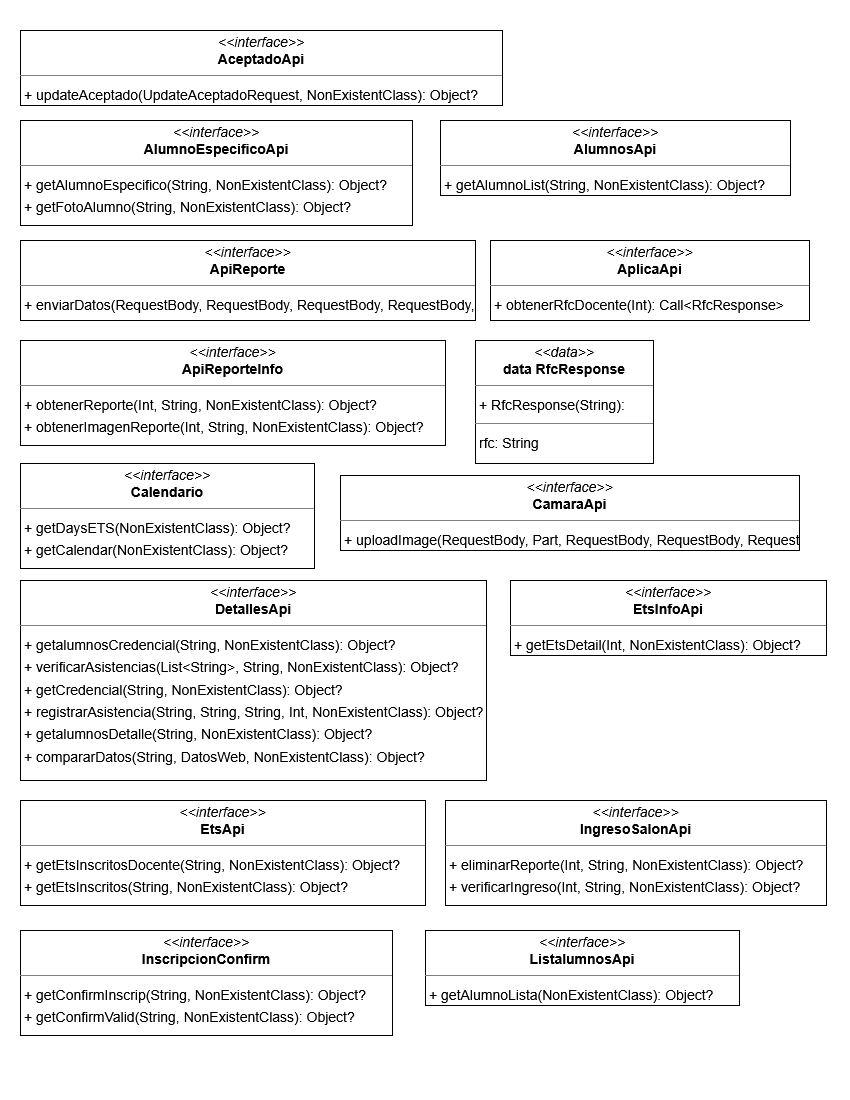
\includegraphics[width=0.75\textwidth]{DiagramasMoviles/DCM (10)}
		\caption{Diagrama de clases para package Retrofit parte 1.}
		\label{fig:Retrofit1}
	\end{center}
\end{figure}

\newpage

\subsection{Diagrama de clases de package Retrofit parte 2}

La Figura \ref{fig:Retrofit2} muestra la segunda parte del diagrama de clases de package Retrofit.

\begin{figure}[htbp!]
	\begin{center}
		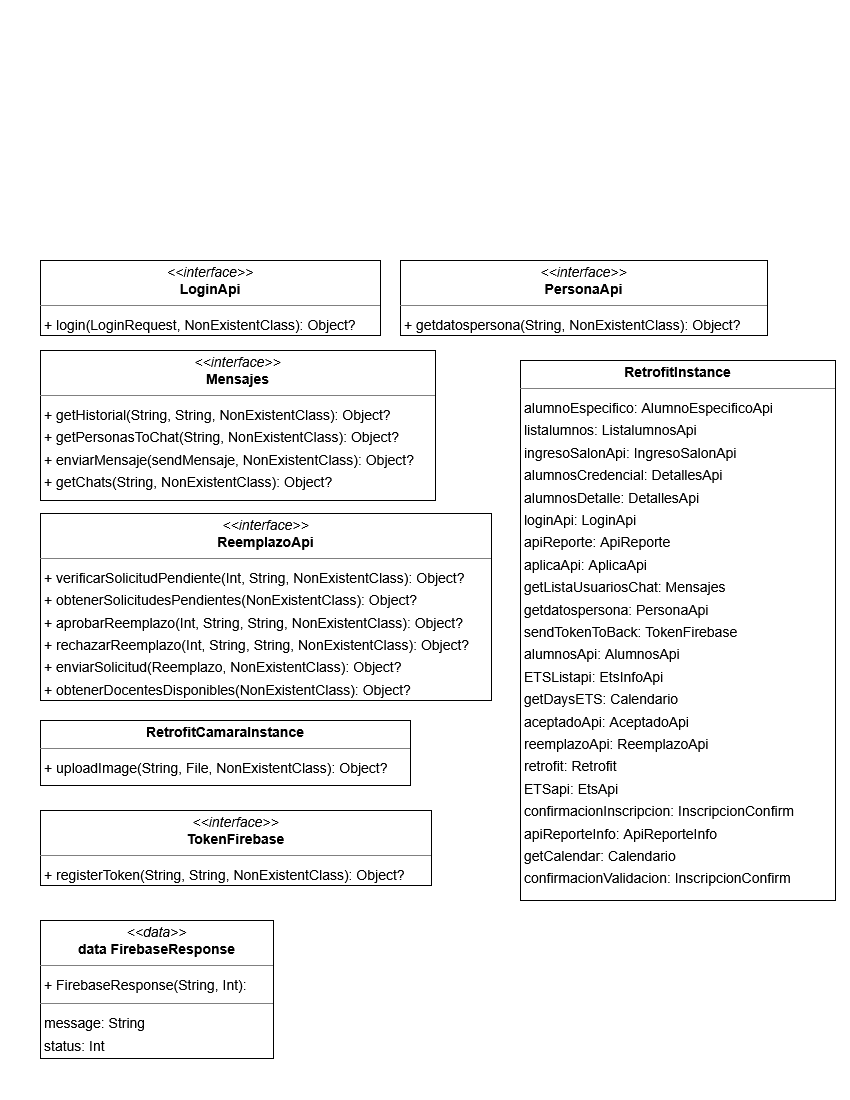
\includegraphics[width=0.75\textwidth]{DiagramasMoviles/DCM (11)}
		\caption{Diagrama de clases para package Retrofit parte 2.}
		\label{fig:Retrofit2}
	\end{center}
\end{figure}

\newpage